\documentclass[a4paper,11pt]{article}

\usepackage[T1]{fontenc}
\usepackage[utf8]{inputenc}
\usepackage{graphicx}
\usepackage{xcolor}

\renewcommand\familydefault{\sfdefault}
\usepackage{tgheros}
\usepackage[defaultmono]{droidmono}

\usepackage{amsmath,amssymb,amsthm,textcomp}
\usepackage{enumerate}
\usepackage{multicol}
\usepackage{tikz}

\usepackage{geometry}
\geometry{left=25mm,right=25mm,%
bindingoffset=0mm, top=20mm,bottom=20mm}


\linespread{1.3}

\newcommand{\linia}{\rule{\linewidth}{0.5pt}}

% custom theorems if needed
\newtheoremstyle{mytheor}
    {1ex}{1ex}{\normalfont}{0pt}{\scshape}{.}{1ex}
    {{\thmname{#1 }}{\thmnumber{#2}}{\thmnote{ (#3)}}}

\theoremstyle{mytheor}
\newtheorem{defi}{Definition}

% my own titles
\makeatletter
\renewcommand{\maketitle}{
\begin{center}
\vspace{1ex}
{\small \textsc{\@title}}
\vspace{1ex}
\\
% \linia\\
% \vspace{1ex}
\end{center}
}
\makeatother
%%%

\usepackage{titlesec}

\titleformat*{\section}{\small\bfseries}

% custom footers and headers
\usepackage{fancyhdr}
% \pagestyle{fancy}
% \lhead{}
% \chead{}
% \rhead{}
% \lfoot{}
% \cfoot{}
% \rfoot{Page \thepage}
% \renewcommand{\headrulewidth}{0pt}
% \renewcommand{\footrulewidth}{0pt}
%
\usepackage{amsmath}
\usepackage{siunitx}
\usepackage{graphicx}
\usepackage{multicol}
% code listing settings
\usepackage{listings}
\lstset{
    language=Python,
    basicstyle=\ttfamily\small,
    aboveskip={1.0\baselineskip},
    belowskip={1.0\baselineskip},
    columns=fixed,
    extendedchars=true,
    breaklines=true,
    tabsize=4,
    prebreak=\raisebox{0ex}[0ex][0ex]{\ensuremath{\hookleftarrow}},
    frame=lines,
    showtabs=false,
    showspaces=false,
    showstringspaces=false,
    keywordstyle=\color[rgb]{0.627,0.126,0.941},
    commentstyle=\color[rgb]{0.133,0.545,0.133},
    stringstyle=\color[rgb]{01,0,0},
    numbers=left,
    numberstyle=\small,
    stepnumber=1,
    numbersep=10pt,
    captionpos=t,
    escapeinside={\%*}{*)}
}

%%%----------%%%----------%%%----------%%%----------%%%

\begin{document}

\title{Stats Mid-Term Assignment | Rvail Naveed: 17321983}

\date{26/03/2020}

\maketitle

\begin{minipage}[t]{0.48\linewidth}
    \section*{Q1(a)}
        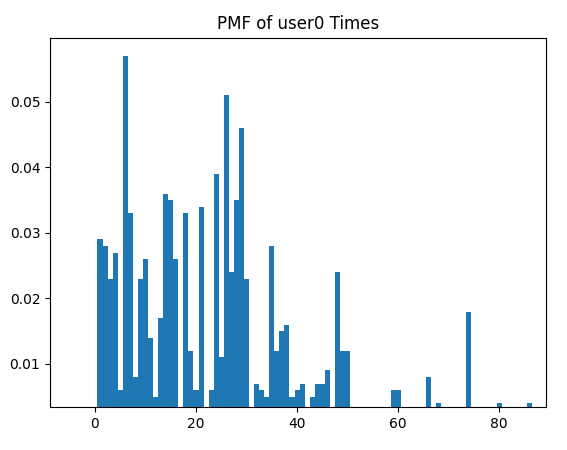
\includegraphics[scale=0.3]{pmf.png}
\end{minipage}
\hfill
\begin{minipage}[t]{0.48\linewidth}
    \section*{Q1(b)} 
        Mapping the values for $X_0$ to all the values for user0 we get
        582 values where $X_0=1$. Since $Prob(X_0 = 1) = E[X_0]$. We can use the formula for empirical mean:
        $$ \frac{1}{N}\sum_{k=1}^NX_k = \frac{582}{1000}$$
        $Prob(X_0 = 1) = 0.582$
    \newline
    \section*{Q1(d)} 
        Code in appendix
\end{minipage}

\section*{Q1(c)} 
    Chebyshev: 
    \begin{itemize}
        \item Gives full distribution of $X_0$
        \item Only requires mean and variance to full describe distribution
        \item Con: Approximation when N is finite, hard to determine accuracy
    \end{itemize}
    $$ \mu = 0.582,  \sigma = \sqrt{\mu(1-\mu)} = 0.493, N=1000 $$
    $$ \mu - \frac{\sigma}{\sqrt{0.05N}} \leq X_0 \leq \mu + \frac{\sigma}{\sqrt{0.05N}} = 0.582 - \frac{0.493}{\sqrt{0.05(1000)}} \leq X_0 \leq 0.582 + \frac{0.493}{\sqrt{0.05(1000)}}$$ 
    $$ 0.512 \leq X_0 \leq 0.651 $$ 

    CLT:
    \begin{itemize}
        \item Provides an actual bound and not an approximation
        \item Works for all N
        \item Con: It's loose in general
    \end{itemize}
    $$ \frac{\frac{(X_1+X_2+...+X_n)}{n} - \mu}{\frac{\sigma}{\sqrt{n}}}  = $$

    Bootstrapping:
    \begin{itemize}
        \item Gives full distribution without assuming normality
        \item Con: Approximation when N is finite, hard to determine accuracy
        \item Con: Requires the availability of all N measurements
    \end{itemize}
    $$ $$
\section*{Q2}
    \textbf{user1}: 0.416 | \textbf{user2}: 0.399 | \textbf{user3}: 0.334


\section*{Q3}
    Using marginalisation and summing all the probabilites to get $Z_n$:
    $$ P(X_0 = 1)P(U_0) + P(X_1 = 1)P(U_1) + P(X_2 = 1)P(U_2) + P(X_3 = 1)P(U_3) $$
    $$ 0.582(0.09742...) + 0.416(0.40468...) + 0.399(0.23529...) + 0.334(0.26260...) $$
    $ Z_n = 0.4066392298682297 $

\section*{Q4}
    $$ P(U_n=0|Z_n > 10ms) = P(E|F) = \frac{P(F|E)P(E)}{P(F)} $$
    \begin{itemize}
        \item $ P(F|E) = 0.582 $ (from Q1)
        \item $ P(E) = 0.09742483650256 $ (from top line of dataset)
        \item $ P(E^c) = 1-P(E) = 1-0.09742483650256 = 0.902575163 $
        \item $ P(F|E^c) = 1-P(F|E) = 1-0.582 = 0.418 $
        \item $ P(F) = P(F|E)*P(E) + P(F|E^c)*P(E^c) $
    \end{itemize}

    $$ P(U_n=0|Z_n > 10ms) = \frac{0.582 * 0.09742483650256}{(0.582 * 0.09742483650256)+(0.418*0.902575163)} $$
    $ P(U_n=0|Z_n > 10ms) = 0.1306547741392685 $
\end{document}